% ================================================================================================================
%
% ________/\\\\\\\\\_____/\\\\\\\\\_____/\\\\\\\\\\\\\\\__/\\\\\\\\\\\_____/\\\\\\\\\__________________        
%  _____/\\\////////____/\\\\\\\\\\\\\__\///////\\\/////__\/////\\\///____/\\\\\\\\\\\\\________________       
%   ___/\\\/____________/\\\/////////\\\_______\/\\\___________\/\\\______/\\\/////////\\\_______________      
%    __/\\\_____________\/\\\_______\/\\\_______\/\\\___________\/\\\_____\/\\\_______\/\\\__/\\\\\\\\\\\_     
%     _\/\\\_____________\/\\\\\\\\\\\\\\\_______\/\\\___________\/\\\_____\/\\\\\\\\\\\\\\\_\///////////__    
%      _\//\\\____________\/\\\/////////\\\_______\/\\\___________\/\\\_____\/\\\/////////\\\_______________   
%       __\///\\\__________\/\\\_______\/\\\_______\/\\\___________\/\\\_____\/\\\_______\/\\\_______________  
%        ____\////\\\\\\\\\_\/\\\_______\/\\\_______\/\\\________/\\\\\\\\\\\_\/\\\_______\/\\\_______________ 
%         _______\/////////__\///________\///________\///________\///////////__\///________\///________________
%
% _____/\\\\\\\\\\\\__/\\\\\\\\\\\\_____/\\\\____________/\\\\__/\\\_____________        
%  ___/\\\//////////__\/\\\////////\\\__\/\\\\\\________/\\\\\\_\/\\\_____________       
%   __/\\\_____________\/\\\______\//\\\_\/\\\//\\\____/\\\//\\\_\/\\\_____________      
%    _\/\\\____/\\\\\\\_\/\\\_______\/\\\_\/\\\\///\\\/\\\/_\/\\\_\/\\\_____________     
%     _\/\\\___\/////\\\_\/\\\_______\/\\\_\/\\\__\///\\\/___\/\\\_\/\\\_____________    
%      _\/\\\_______\/\\\_\/\\\_______\/\\\_\/\\\____\///_____\/\\\_\/\\\_____________   
%       _\/\\\_______\/\\\_\/\\\_______/\\\__\/\\\_____________\/\\\_\/\\\_____________  
%        _\//\\\\\\\\\\\\/__\/\\\\\\\\\\\\/___\/\\\_____________\/\\\_\/\\\\\\\\\\\\\\\_ 
%         __\////////////____\////////////_____\///______________\///__\///////////////__
%
% ________________________________________________________________________________________________________________________        
%  ________________________________________________________________________________________________________________________       
%   ___/\\\\\\\\______________________________________________________________________/\\\_______________________/\\\__/\\\_      
%    __/\\\////\\\_____/\\\\\\\\______/\\\\\_______/\\\\\__/\\\\\_______/\\\\\\\\___/\\\\\\\\\\\__/\\/\\\\\\\____\//\\\/\\\__     
%     _\//\\\\\\\\\___/\\\/////\\\___/\\\///\\\___/\\\///\\\\\///\\\___/\\\/////\\\_\////\\\////__\/\\\/////\\\____\//\\\\\___    
%      __\///////\\\__/\\\\\\\\\\\___/\\\__\//\\\_\/\\\_\//\\\__\/\\\__/\\\\\\\\\\\_____\/\\\______\/\\\___\///______\//\\\____   
%       __/\\_____\\\_\//\\///////___\//\\\__/\\\__\/\\\__\/\\\__\/\\\_\//\\///////______\/\\\_/\\__\/\\\__________/\\_/\\\_____  
%        _\//\\\\\\\\___\//\\\\\\\\\\__\///\\\\\/___\/\\\__\/\\\__\/\\\__\//\\\\\\\\\\____\//\\\\\___\/\\\_________\//\\\\/______ 
%         __\////////_____\//////////_____\/////_____\///___\///___\///____\//////////______\/////____\///___________\////________
%
% __/\\\_____________________________/\\\\\\____________/\\\_______________________________        
%  _\/\\\____________________________\////\\\___________\/\\\_______________________________       
%   _\/\\\_______________________/\\\____\/\\\___________\/\\\_______________________________      
%    _\/\\\_________/\\\____/\\\_\///_____\/\\\___________\/\\\______/\\\\\\\\___/\\/\\\\\\\__     
%     _\/\\\\\\\\\__\/\\\___\/\\\__/\\\____\/\\\______/\\\\\\\\\____/\\\/////\\\_\/\\\/////\\\_    
%      _\/\\\////\\\_\/\\\___\/\\\_\/\\\____\/\\\_____/\\\////\\\___/\\\\\\\\\\\__\/\\\___\///__   
%       _\/\\\__\/\\\_\/\\\___\/\\\_\/\\\____\/\\\____\/\\\__\/\\\__\//\\///////___\/\\\_________  
%        _\/\\\\\\\\\__\//\\\\\\\\\__\/\\\__/\\\\\\\\\_\//\\\\\\\/\\__\//\\\\\\\\\\_\/\\\_________ 
%         _\/////////____\/////////___\///__\/////////___\///////\//____\//////////__\///__________
%
% ================================================================================================================

\section{Инструментарий ``CATIA-GDML geometry builder''}\label{sec:secBuilder}

``CATIA-GDML geometry builder'' (далее просто ``Builder'') представляет собой набор документов-шаблонов и макропрограмм для САПР CATIA~v5 вместе с настройками окружения и инструкциями к применению стандартных средств CATIA~v5. ``Builder'' ставит своей задачей упростить процесс создания CSG моделей с иерархией объёмов, напрямую совместимых с GEANT/ROOT.

Центральная идея ``Builder'' заключается в правилах соответствия сущностей CATIA~v5 и сущностей геометрии в GEANT/ROOT. Это соответствие делает возможным конвертацию MC-модели в CATIA~v5 в любой внешний файл с целью дальнейшего импорта в GEANT/ROOT. В качестве формата для обмена был выбран XML-подобный формат GDML (geometry description markup language, см. секцию~\ref{sec:secGDML}), разработанный в CERN, для которого в GEANT4 и ROOT реализованы методы импорта и экспорта.

Вся геометрия установки создаётся в одном документе типа CATProduct. Объёму соответствует деталь, хранящаяся в файле типа CATPart. Форме соответствует главное тело детали, по умолчанию называемое PartBody. В CATIA не записывается описание материала так, как это принято в GEANT/ROOT, а сохраняется только имя материала в пользовательском параметре Material. Это возможно по той причине, что существует практика хранить описание материалов во внешнем файле или базе данных, считывать его перед выполнением моделирования и приписывать объёмам в соответствии с именами. Для обозначения физического объёма $B$ внутри $A$ в структуре документа, описывающего объём $A$, создаются тела Body.B.*, где * по умолчанию обозначает номер вхождения, но допускается запись любой идентифицирующей строки.

% \textbf{Может быть частично перенести в описание методов описания геометрии в GEANT/ROOT.}
% done
Также в ``Builder'' предусмотрена возможность задания геометрии некоторыми продвинутыми методами, специфичными для GEANT/ROOT, см. секции~\ref{sec:secAssemblyVolume}, \ref{sec:secDivisionReplica}.

Один из плюсов ``Builder'' заключается в том, что пользователю предоставляется возможность работать с полноценной инженерной моделью и MC-моделью в одной и той же среде, имеющей широкие возможности для анализа и редактирования геометрии. ``Builder'' не ставит своей задачей перевод модели из одного геометрического представления в другой, но значительно ускоряет процесс создания одной геометрии, на основе другой. Также важно отметить, что подходы к геометрическому моделированию в САПР подразумевают широкое использование параметров --- практически все размеры, значения поворотов и сдвигов, количество вхождений в массивы и прочие числа, определяющие форму и структуру модели, могут подвергаться изменению на любом этапе. Если в процесе построения модели этот принцип параметризированного моделирования нарушается, САПР предупреждает пользователя перед выполнением операции, которая приведёт к разрыву связи с параметром. В CATIA~v5 при изменении каких-либо параметров геометрическая модель перестраивается интерактивно --- от долей секунды до нескольких секунд в зависимости от сложности модели.  Эта стандартная черта САПР очень удобна при работе с MC-моделями и отсутствует, например, в GEANT и ROOT.

``Builder'' включает в себя файлы, в которых специальным образом построены примитивы GEANT/ROOT, позволяющие пользователю при построении MC-модели не вникать в подробности реализации, а использовать их практически как и в процессе создания геометрии средствами ROOT или GEANT. ``Builder'' также включает в себя макропрограммы для CATIA~v5, которые также ставят своей задачей сделать процесс построения геометрии в ``Builder'' максимально похожим на процесс построения геометрии в GEANT или ROOT. Основной макрос --- это конвертер \macroname{CATIA2GDML}, который проецирует дерево построения модели в CATIA в GDML файл. Также разработан обратный конвертер \macroname{GDML2CATIA} для импорта GDML файлов.

Целевая аудитория ``CATIA-GDML geometry builder'' --- физики, владеющие CATIA~v5 на базовом уровне, и инженеры, продвинутые пользователи САПР, изучившие способ представления геометрии в GEANT/ROOT хотя бы на теоретическом уровне. \textbf{Есть опыт, который показывает, что для достижения такого уровня как физикам, так и инженерам, достаточно прохождения двухнедельного курса.}

Предлагается новый алгоритм работы, в котором ``Builder'' используется как многофункциональный инструмент. Описанный ниже алгоритм сформулирован на успешном опыте разработки CBM RICH на протяжении 3 (4) лет.

Задача создания и поддержания актуальной MC-модели поручается ответственному человеку, владеющему CATIA~v5, GEANT/ROOT и ``CATIA-GDML geometry builder''. В зависимости от того, какая информация и в каких файлах имеется к началу работы, алгоритм немного различается.
% case 1
Если разработка ведётся в нуля и нет никаких данных в ЭВМ, что возможно, например, когда проект находится на таком этапе, когда нужно выполнить грубое моделирование, показывающее принципиальную возможность реализации, то наиболее оптимальный способ --- сразу строить MC-модель в CATIA~v5 средствами ``Builder'' (см. секцию~\ref{sec:secMCfromScratch}).
% case 2
Если, скажем, проект находится на раннем этапе разработки и уже имеется какая-то приблизительная САПР модель, то рекомендуется импортировать её стандартными средствами CATIA~v5, чтобы затем на её основе построить MC-модель в CATIA в автоматизированном режиме с помощью средств ``Builder''. Более подробно этот случай описан в секции~\ref{sec:secMCfromCAD}.
% case 3
Третий распространённый случай это когда уже имеется некоторая MC-модель в конечной системе моделирования. В этом случае можно импортировать модель в CATIA в MC-формате, однако иногда требуются некоторые дополнительные ручные операции после импорта. Они выполняются однократно и лишь делают структуру документа более оптимальной, но не изменяют геометрию. Этот случай описан в секции~\ref{sec:secMCtoCAD}.

Во всех этих алгоритмах, независимо от типа и количества исходных данных, получаются файлы CATIA в формате ``Builder'', которые в дальнейшем будут являться основными (первичными) файлами для получения рабочей MC-модели в экспериментальном пакете, которым в случае CBM RICH является CbmRoot. Модель из CATIA экспортируется в GDML файл, который не требует каких-либо последующих изменений в структуре. Для достижения этого условия была проведена огромная работа по мере разработки MC-модели CBM RICH. Допускается и даже рекомендуется текстовое редактирование GDML файла, но только для изменения значений параметров в define секции у параметризованных моделей. Затем, по желанию коллаборации, GDML файл может быть конвертирован в бинарный ROOT-файл, который содержит геометрию, которую невозможно редактировать. Это защищает модель от случайных изменений, что особенно актуально в случае параметризованных моделей. Соответственно, если требуется изменить значения параметров, пользователь может отредактировать GDML файл и экспортировать в новый ROOT файл. Практика показывает, что в случае, если требуется множество файлов с MC-геометрией, то обязательно нужно писать комментарии --- либо в самом GDML файле, либо в текстовом файле рядом с GDML/ROOT файлом. Обычно в коллаборации вводят правила именования файлов.

% ================================================================================================================
%  ____            _                                                   
% |  _ \  ___  ___(_) __ _ _ __      _ __  _ __ ___   ___ ___  ___ ___ 
% | | | |/ _ \/ __| |/ _` | '_ \    | '_ \| '__/ _ \ / __/ _ \/ __/ __|
% | |_| |  __/\__ \ | (_| | | | |   | |_) | | | (_) | (_|  __/\__ \__ \
% |____/ \___||___/_|\__, |_| |_|   | .__/|_|  \___/ \___\___||___/___/
%                    |___/          |_|                                
% ================================================================================================================

\subsection{Поддержка MC-модели с помощью ``Builder'' на протяжении процесса проектирования детектора}\label{sec:DesignProcess}

Использование ``Builder'' для создания и поддержки MC-геометрии на этапе проектирования детектора имеет некоторые особенности. Инженерный проект изменяется и необходимо постоянно поддерживать соответствие MC-модели и САПР-модели. В процессе проектирования можно выделить два вида изменений --- радикальные перемены в структуре и уточнение существующих узлов. В первом случае нередко бывает удобно с нуля перестроить MC-модель, может быть используя некоторые созданные ранее подсборки. Тогда достаточно выделить повторно используемые файлы, описывающие некоторые объёмы, и вставить их в качестве компонентов в верхний документ типа CATProduct разрабатываемой новой геометрии. Если между документами существовала связь типа дочерний-материнский, то она нарушится, т.к. изменится контекст. Для восстановления достаточно выполнить операцию автоматического переопределения связей с помощью операции define contextual links.

В процессе уточнения геометрии иногда возникает необходимость вводить какие-то особенности, которые приводят к невозможности использовать принципы многократного позиционирования объёмов, такие как деление объёмов (секция~\ref{sec:secDivisionReplica}) и массивы (\todo ссылка). Тогда приходится нарушать периодичность структуры, и следовательно краткость описания, и использовать независимые вхождения дочерних объёмов. 

В качестве примера можно привести фокусирующую систему CBM RICH, состоящую из 80~сегментов зеркал шести типов. Для наиболее эффективного описания подобной геометрии следует использовать деление объёма (см. секцию~\ref{sec:secMacroReplica} \todo может быть будет ссылка на секцию про реплику, но не макрос \todo), имеющего форму примитива типа sphere, вдоль кругового направления. Известно, что если использовать деление объёмов, то получается геометрия, более оптимальная с точки зрения времени моделирования прохождения частиц. Исходя из этих соображений, на раннем этапе зеркала фокусирующей системы CBM RICH были созданы следующим образом. Каждое из двух зеркал состояло из трёх сегментов сферы, вытянутых вдоль горизонтальной оси, разделённых на 10~долей вдоль кругового направления, и ещё одной горизонтальной полосы, в которой отдельные сегменты зеркал вставлялись независимо. Дольки, полученные делением каждого из трёх сегментов сферы, соответствуют трём типам сегментов зеркал. 

\begin{minipage}[t]{0.495\textwidth}
\begin{figure}[H]
\centering
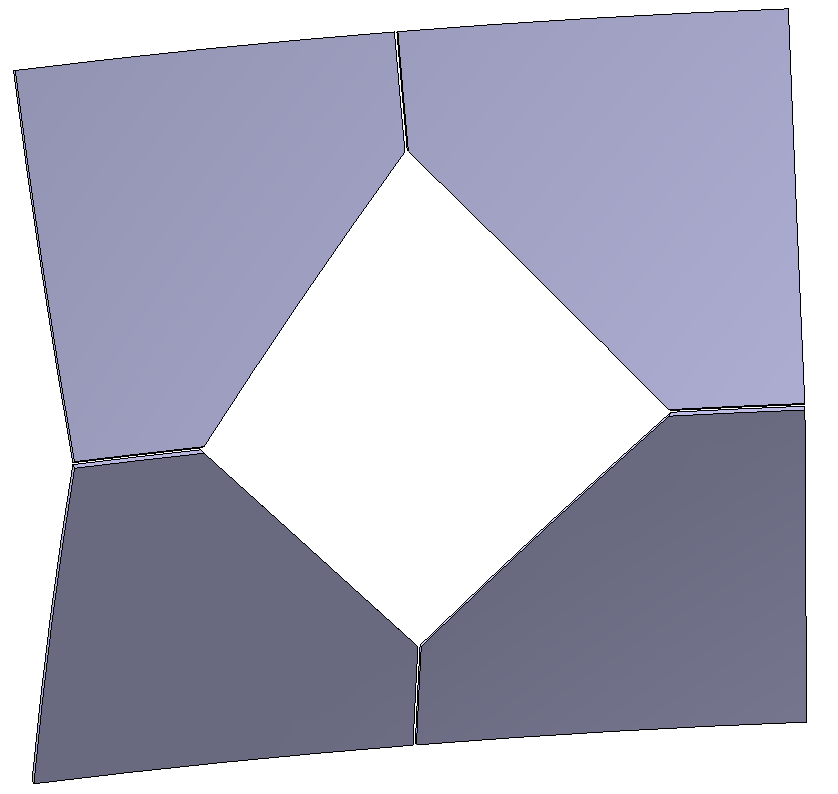
\includegraphics[width=0.7\textwidth]{pictures/Mirror_tiles_special.png}
\caption{Особые сегменты зеркал (type4 и type5), имеющие вырез для ионопровода.}
\label{fig:SpecialMirrorTiles}
\end{figure}
\end{minipage}
\hspace{0.01\textwidth}
\begin{minipage}[t]{0.495\textwidth}
В последней полосе, наиболее близкой к пучку, не было возможности также использовать деление объёма из-за наличия прорези для пучковой трубы. Это привело к тому, что помимо четвёртого типа сегментов зеркал, было введено два дополнительных типа сегментов зеркал, имеющих симметричную форму (см.~\figref{fig:SpecialMirrorTiles}). При таком описании между сегментами зеркал отсутствуют зазоры. Они не были реализованы, т.к. на том этапе эта подробность не имела значения, однако присутствовала возможность легко их добавить введя один дополнительный уровень вложенности.
\end{minipage}

\bigskip

К какой-то момент по мере проработки проекта детектора были зафиксированы параметры зеркал --- радиус, количество и форма сегментов, угол наклона, положение центра, и т.д. Также возникла необходимость выполнять моделирование отклонения индивидуальных сегментов от идеального положения (см. секцию~\ref{sec:secRICHgeoMirrorMis}). Для такого моделирования пользователь должен иметь возможность для каждого сегмента задавать углы отклонения вокруг двух осей в локальной системе координат, индивидуальной для каждого отдельного сегмента. Это требование противоречит идее деления объёмов, где все дольки, полученные в результате деления, имеют одинаковую форму, расположены строго периодически вдоль заданного направления с некоторым шагом и полностью заполняют пространство разделяемого объёма. В случае деления вдоль кругового направления дольки отличаются углом поворота вокруг оси Z и невозможно  задать какое-либо дополнительное вращение каждой отдельной дольке. Таким образом, пришлось отказаться от использования деления объёмов и использовать независимое многократное позиционирование сегментов внутри объёма-контейнера.

% ================================================================================================================
%  ____       _           _ _   _                
% |  _ \ _ __(_)_ __ ___ (_) |_(_)_   _____  ___ 
% | |_) | '__| | '_ ` _ \| | __| \ \ / / _ \/ __|
% |  __/| |  | | | | | | | | |_| |\ V /  __/\__ \
% |_|   |_|  |_|_| |_| |_|_|\__|_| \_/ \___||___/
%                                                
% ================================================================================================================

\subsection{Примитивы в ``Builder''}\label{sec:Primitives}

%В принципе мотивация уже обсуждалась в секции выше.
Любой примитив можно построить стандартными средствами САПР, используя эскизы и формообразования, но в таком случае конвертер не сможет автоматически определить, является ли построенная форма примитивом и, если да, определить параметры примитива. По этой причине был разработан принцип хранения формы примитива в MC-модели с помощью средства CATIA~v5, называемого User-Defined Feature (UDF), и средства для автоматизации создания примитивов --- макросы \macroname{AddShape} и \macroname{Poly}. Каждый примитив реализован в своём файле типа CATPart, в котором создаётся описание UDF, превращая этот файл в шаблон. Некоторые объекты модели, в случае примитивов --- некоторые стандартные плоскости, и параметры модели объявляются <<внешними>>. Далее в другом документе возможно создать вхождение формы, определённой в файле-шаблоне, вызвав соответствующее формообразование. При этом в текущем документе потребуется лишь выбрать необходимые элементы, с которыми будут совпадать <<внешние>> объекты шаблона, и задать значения параметрам создаваемого вхождения. Примитивы в ``Builder'' построены так, чтобы этими совпадающими элементами были стандартные плоскости. За счёт этого при создании вхождения достаточно нажать кнопку use identical names и CATIA автоматически совместит правильные элементы. Более того, использование макроса \macroname{AddNewPart} автоматизирует этот процесс.

В ``CATIA-GDML geometry builder'' с помощью UDF реализованы следующие примитивы:

% ссылка на: https://root.cern.ch/root/htmldoc/guides/users-guide/Geometry.html#primitive-shapes

\begin{itemize}
\itemsep0pt
\item arb8 --- arbitrary 8 vertices shape;
\item box --- прямоугольный параллелепипед;
\item cons --- сектор конуса (cone segment);
\item ellipsoid --- эллипсоид;
\item elliptical cone --- эллиптический конус;
\item elliptical tube --- эллиптический цилиндр;
\item orb --- шар (полный);
\item para --- параллелепипед общего вида (parallelepiped);
\item sphere --- сектор полого шара;
\item torus --- сектор открытого тора;
\item trap --- трапецоид общего вида (general trapezoid);
\item trd --- трапецоид частного вида (trapezoid);
\item tubs --- сектор полого цилиндра (tube section);
\item twisted box --- скрученный прямоугольный параллелепипед;
\item twisted trap --- скрученный трапецоид общего вида (twisted general trapezoid);
\item twisted trd --- скрученный трапецоид частного вида (twisted trapezoid);
\item twisted tubs --- скрученный сектор полого цилиндра (twisted tube section).
\end{itemize}

Из-за того, что полипримитивы polycone и polyhedra имеют переменное число секций, оказалось невозможным реализовать их так же как и остальные примитивы с помощью UDF. Чтобы представить полипримитив в дереве построения модели в CATIA используется последовательность чередующихся UDF, описывающих отдельные секции, и формообразований translate, необходимых для обеспечения сдвига секций относительно друг друга. В случае polycone секция моделируется стандартный примитивом cons, а для polyhedra аналогичной стандартной формы не существует, поэтому она была введена искусственно. Примитив hedra существует только в ``Builder'', он нужен для создания polyhedra и не можетбыть использован где-либо ещё.

Рассмотрим реализацию примитива Tubs (tube section) в файле-шаблоне UDF системы CATIA.

Примитив Tubs имеет 5 параметров --- радиусы внутренней $r_{min}$ и внешней $r_{max}$ цилиндрических поверхностей, половина высоты примитива $dz$ вдоль оси $Z$, начальный угол вращения $pSPhi$ и диапазон по углу $pDPhi$, откладываемые против часовой стрелки от оси $X$.

% (также на ~\figref{fig:TubsCases} (1))

На~\figref{fig:TubsUDF} приведён документ-шаблон со стандартной комбинацией параметров, соответствующей наиболее общему случаю примитива Tubs. На~\figref{fig:TubsCases} приведены <<особые>> формы примитива Tubs, имеющие отличную топологию геометрии, и получающиеся при некоторых комбинациях значений параметров.
Если $r_{min}=0$, то внутренняя цилиндрическая поверхность вырождается (случаи 2 и 4).
Если $pDPhi = 360$, то плоские грани сливаются образуя либо полный цилиндр (случай 4) либо кольцо (случай 3).

\begin{figure}[H]
\centering
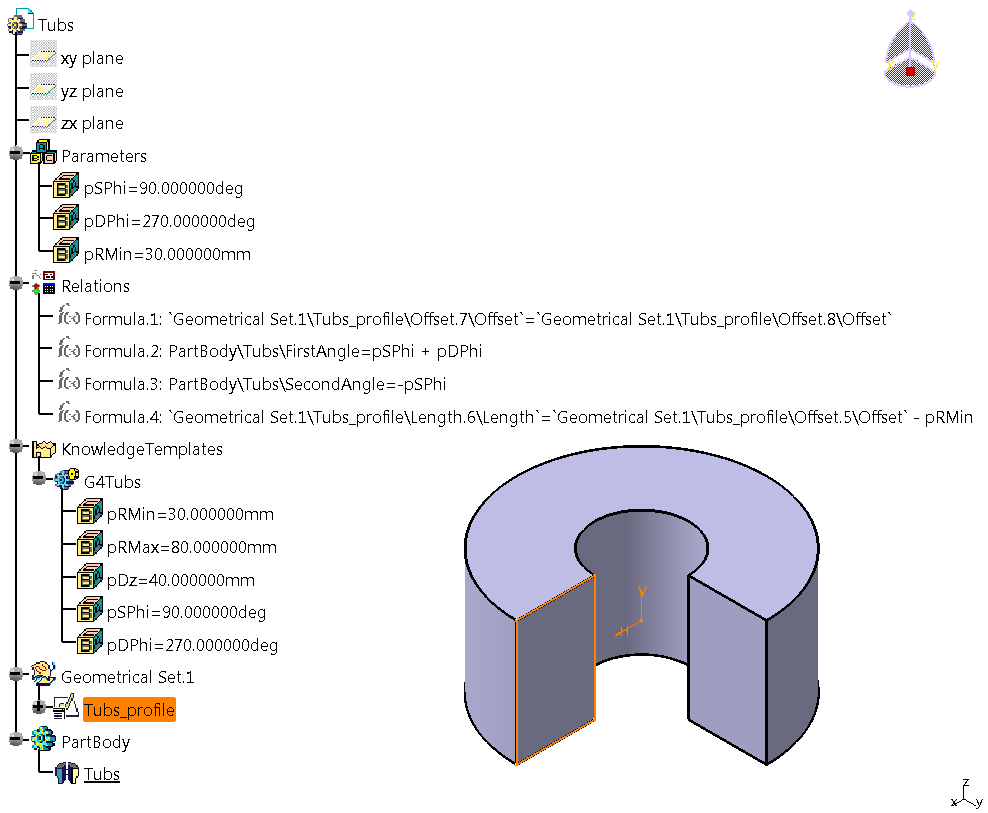
\includegraphics[width=0.7\textwidth]{pictures/Tubs_UDF_file.png}
\caption{Примитив Tubs в файле-шаблоне CATIA.}
\label{fig:TubsUDF}
\end{figure}

\begin{figure}[H]
\centering
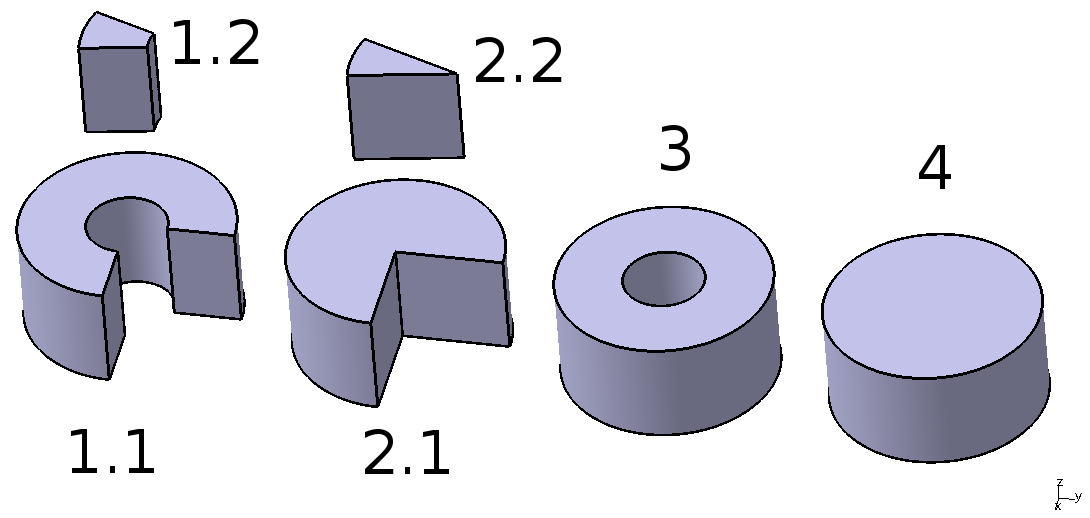
\includegraphics[width=0.7\textwidth]{pictures/Tubs_cases_2.png}
\caption{Примитив Tubs (Tube section) в файле-шаблоне CATIA.}
\label{fig:TubsCases}
\end{figure}

Все эти формы получаются автоматически из базового принципа построения примитива.
Для получения формы примитива Tubs с помощью САПР необходимо выполнить формообразование вращения прямоугольного профиля вокруг оси, находящейся в плоскости профиля и параллельной одной из сторон профиля.

Не допускаются следующие комбинации:
$r_{min} = r_{max}$ --- примитив вырождается в тонкую поверхность.
$r_{min} > r_{max}$ --- САПР построит форму, в которой поменяются местами внутренняя и внешняя повехрность, однако поведение системы проведения частицы не определено.
$r_{max} = 0$ (из правила $r_{min} < r_{max}$ это подразумевает, что $r_{min} = r_{max} = 0$) --- примитив вырождается в отрезок на оси.
$dz = 0$ --- примитив вырождается в фигуру на плоскости (круг, сектор круга, кольцо или сектор кольца в зависимости от значений остальных параметров).

Описанный файл-шаблон вызывается при построении формы и пользователь не видит подробностей его реализации --- ему доступен лишь список управляющих параметров (см.~\figref{fig:UDFinstance}).

\begin{figure}[H]
\centering
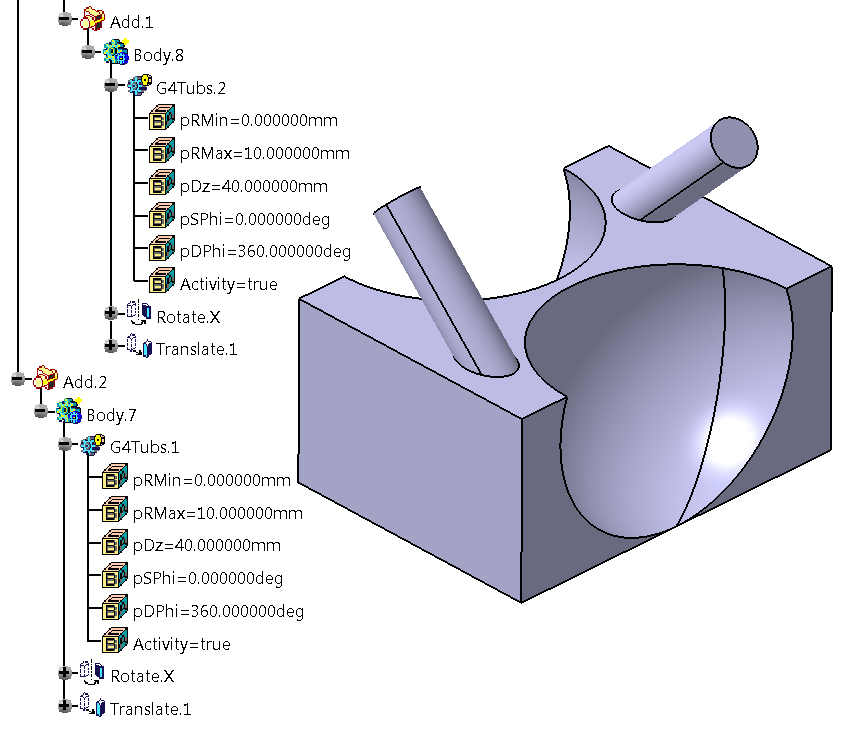
\includegraphics[width=0.5\textwidth]{pictures/UDF_instance.png}
\caption{Примитив Tubs, созданный с помощью UDF из файла-шаблона.}
\label{fig:UDFinstance}
\end{figure}


\bigskip

% UDF с rule на примере TwistedBox
% \todo проверить

Скрученные примитивы (twisted box, twisted trap, twisted trd, twisted tubs) имеют такую особенность, что при нулевом угле скручивания они превращаются в обычные примитивы (соответственно box, trap, trd и tubs). Для построения скрученных примитивов в CATIA применяется формообразование ``тело по сечениям'', а в качестве направляющей используется спираль, параметры которой зависят от угла скручивания, причём так, что если этот угол равен нулю, то спираль не может быть построена. Для корректной обработки такого исключения применяется возможность CATIA, которая называется rule и позволяет задать программу для того, чтобы выполнять определённые действия при выполнении некоторые условия.
На~\figref{fig:TwistedUDF} приведено ...
\todo

\begin{figure}[H]
\centering
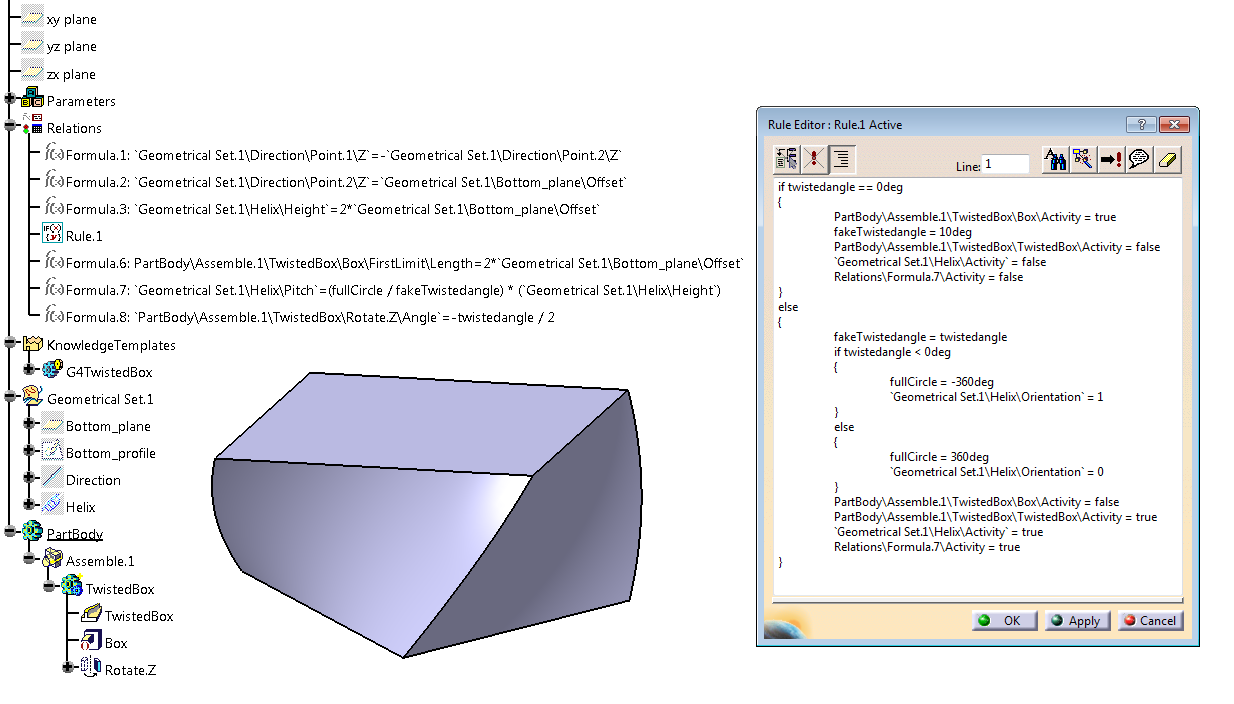
\includegraphics[width=0.9\textwidth]{pictures/Twisted_UDF.png}
\caption{Примитив TwistedBox, в котором применяется rule.}
\label{fig:TwistedUDF}
\end{figure}

\bigskip

% ================================================================================================================
%  ____              _                  
% | __ )  ___   ___ | | ___  __ _ _ __  
% |  _ \ / _ \ / _ \| |/ _ \/ _` | '_ \ 
% | |_) | (_) | (_) | |  __/ (_| | | | |
% |____/ \___/ \___/|_|\___|\__,_|_| |_|
%                                       
% ================================================================================================================

\subsection{Булевы операции}\label{sec:Boolean}

Форма объёма может быть задана как примитив либо Булева операция над примитивами или результатами Булевых операций (см.~\ref{sec:secGeoCSG}), причём работает такое правило, что первый операнд каждой операции не должен подвергаться каким-либо преобразованиям координат. При создании Булевых операции матрица позиционирования второго операнда относительно первого задаётся трёмя поворотами вокруг стандартных фиксированных осей и одним сдвигом --- также, как и при позиционировании дочернего объёма в материнском. Разница заключается в том, что порядок поворотов обратный --- сначала вокруг X, затем вокруг Y и вокруг Z. Сдвиг выполняется после поворотов.

Операндом и результатом Булевой операции в MC-модели в CATIA~v5 по правилам ``Builder'' является тело --- объект типа Body. Для того чтобы создать Булеву операцию необходимо к телу, обозначающему результат, присоединить первый операнд с помощью формообразования Assemble, а второй с помощью одного из формообразований Add, Remove, Intersect в зависимости от типа операции. Если операнд это просто примитив, то в теле будет одно формообразование типа UDF. Второй операнд может также иметь преобразования координат. На~\figref{fig:BooleanComplex} приведён пример формы, составленной четырьмя Булевыми операциями --- два объединения и два вычитания.

\begin{figure}[H]
\centering
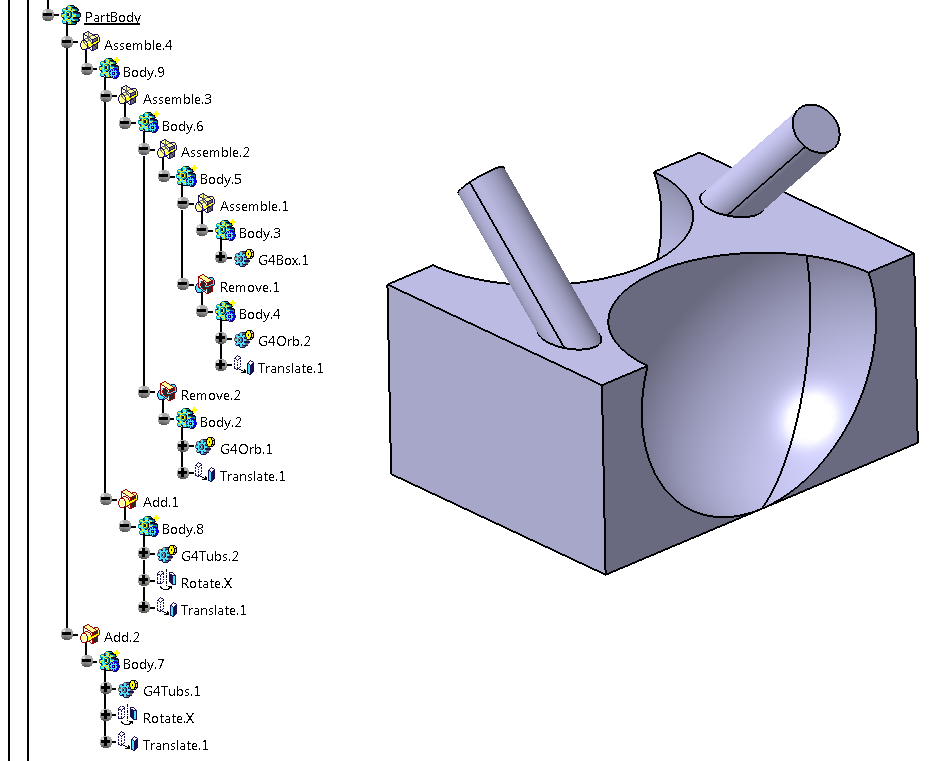
\includegraphics[width=0.9\textwidth]{pictures/Boolean_example.png}
\caption{Форма, составленная Булевой операцией, представленная в CATIA по правилам ``CATIA-GDML geometry builder''.}
\label{fig:BooleanComplex}
\end{figure}

% \todo \textbf{В принципе хочется добавить что-то ещё, но что конкретно?}

% ================================================================================================================
%  ____                                _            _          _   _             
% |  _ \ __ _ _ __ __ _ _ __ ___   ___| |_ ___ _ __(_)______ _| |_(_) ___  _ __  
% | |_) / _` | '__/ _` | '_ ` _ \ / _ \ __/ _ \ '__| |_  / _` | __| |/ _ \| '_ \ 
% |  __/ (_| | | | (_| | | | | | |  __/ ||  __/ |  | |/ / (_| | |_| | (_) | | | |
% |_|   \__,_|_|  \__,_|_| |_| |_|\___|\__\___|_|  |_/___\__,_|\__|_|\___/|_| |_|
%                                                                                
% ================================================================================================================

\subsection{Параметризация}\label{sec:Parameterization}

Одна из наиболее важных возможностей ``CATIA-GDML geometry builder'' --- это возможность создания параметризованных геометрических MC-моделей. У параметризованной модели имеются входные параметры и формулы, задающие зависимость между этими входными параметрами и внутренними переменными, такими как параметры примитивов, значения поворотов и смещений. Данная концепция хорошо ложится на методы работы с геометрией в САПР, особенно CATIA~v5. Также параметризация поддерживается форматом GDML и импортёрами GEANT4 и ROOT.

В модели CATIA~v5 можно вводить пользовательские параметры как в документах типа CATProduct, так и в документах типа CATPart. Причём сборка в CATProduct файле может иметь свои пользовательские параметры и формулы, а дочерние компоненты в CATPart файлах --- свои. Обязательное требование ``Builder'' таково, что все параметры и формулы должны находиться в верхнем продукте. CATIA~v5 позволяет задавать зависимости между любыми параметрами, в том числе внутренними, не являющимися пользовательскими, однако для успешного экспорта в GDML файл формула должна в левой части иметь параметр примитива или угол поворота или значение сдвига, а в правой части --- формулу только над пользовательскими параметрами. Пользовательский параметр CATIA~v5, экспортируемый в переменную в GDML должен обязательно иметь безразмерный тип Real. В связи с этим имеются правила оформления формул и приведения единиц измерения. Также имеется стандартная переменная DEGtoRAD для перевода значения углов из градусов в радианы.

На выходе получается GDML файл, у которого в define секции есть тэги variable, обозначающие входные параметры модели со значениями. При импорте параметризованной геометрии из GDML в ROOT все значения внутренних переменных рассчитываются в соответствии с формулами по значениям входных параметров и параметризация теряется. Следовательно значения входных параметров должны задаваться пользователем непосредственно в GDML файле перед импортом в конечную систему.

% ================================================================================================================
%  _____                  _       _           _ 
% |_   _|__  ___ ___  ___| | __ _| |_ ___  __| |
%   | |/ _ \/ __/ __|/ _ \ |/ _` | __/ _ \/ _` |
%   | |  __/\__ \__ \  __/ | (_| | ||  __/ (_| |
%   |_|\___||___/___/\___|_|\__,_|\__\___|\__,_|
%                                               
% ================================================================================================================

\subsection{Тесселированная геометрия}\label{sec:Tesselated}

\todo см. секцию~\ref{sec:secGeoPoly}

В GEANT/ROOT реализована поддержка триангулированной геометрии, однако специфика этих систем накладывает строгое ограничение --- с помощью треугольников должна быть описана только замкнутая оболочка, ограничивающая область пространства с заданным материалом, т.е. по сути объём.
%Мы знаем юз-кейс.
Для реализации поддержки триангулированной геометрии в ``CATIA-GDML geometry builder'' были разработаны правила её хранения в модели и необходимый код в конвертерах \macroname{CATIA2GDML} и \macroname{GDML2CATIA}.

\todo \textbf{описание реализации в билдере}

% ================================================================================================================
%  ____        _ _     _                                                  
% | __ ) _   _(_) | __| | ___ _ __     _ __ ___   __ _  ___ _ __ ___  ___ 
% |  _ \| | | | | |/ _` |/ _ \ '__|   | '_ ` _ \ / _` |/ __| '__/ _ \/ __|
% | |_) | |_| | | | (_| |  __/ |      | | | | | | (_| | (__| | | (_) \__ \
% |____/ \__,_|_|_|\__,_|\___|_|      |_| |_| |_|\__,_|\___|_|  \___/|___/
%                                                                         
% ================================================================================================================

\subsection{Макропрограммы для CATIA~v5}\label{sec:secMacros}

Макропрограммы для CATIA~v5 написаны на VBA с применением CATIA~API. Все макропрограммы, кроме \macroname{AddShape} и \macroname{Poly}, доступны пользователю в режиме работы над сборкой. В CATIA~v5 различают открытый документ (верхний в дереве в текущем окне), активный документ (синий), выделенный объект (оранжевый) и рабочий объект (подчёркнутый). Пользователь может выполнить все операции, необходимые для получения MC-модели, самостоятельно без применения макропрограмм, но в этом случае велика вероятность упустить какой-либо шаг, что приведёт к ошибке, которую сложно диагностировать.

В MC-модели в CATIA есть строгие правила именования. Применение макросов избавляет пользователя от необходимости контролировать имена объектов в документах. Все имена, сгенерированные при использовании ``Builder'' не конфликтуют между собой и позволяют получить корректный GDML файл на выходе. Практически везде пользователь имеет право изменять суффиксы, не изменяя основного названия, несущего информацию о типе объекта --- формообразования, тела, и т.д. Однако в редких случаях суффикс имеет решающее значение, как например в именах поворотах (напр, ``Rotate.X'') суффикс несёт информацию об оси поворота.

% Вырезан кусок

% Дублирование. Выше уже есть об окружении
Для комфортной работы с ``Builder'' в поставке также имеются файлы для настройки окружения CATIA. Использования окружения в принципе не обязательно, но часть функционала зависит от путей к файлам, которые прописаны в переменных окружения, поэтому настоятельно рекомендуется перед использованием ``Builder'' выполнить настройку, следуя инструкции, поставляемой в пакете.

\subsubsection{\macroname{AddNewPart}}\label{sec:secMacroAddNewPart}

Данная макропрограмма автоматизирует создание нового документа типа CATPart на основе шаблона, содержащего необходимые элементы --- публикация главного тела детали, называемая PartBody, пользовательский параметр под названием Material со значением по умолчанию vacuum. Для удобства работы в файле шаблона и во всех генерируемых новый документах типа CATPart погашены стандартные плоскости. Созданный документ автоматически сохраняется на диск в папку, в которой выполняется построение модели, и которая автоматически определяется из открытого документа типа CATProduct в момент вызова макроса. Путь можно изменить в окне графического интерфейса. Также созданная деталь добавляется в качестве компонента в открытую сборку. Новый документ открывается в дочернем окне CATIA и пользователь может как начать работу над объёмом, так и оставить его пустым и отложить редактирование. Достаточно закрыть это окно и система перейдёт обратно к редактированию сборки.

\subsubsection{\macroname{AddShape}}\label{sec:secMacroAddShape}

\macroname{AddShape} используется для создания примитивов, в случае необходимости вместе с поворотами и сдвигом. Макропрограмма играет роль интерфейса между пользователем и файлами примитивов. При запуске макроса выводится окно со списком доступных примитивов, по нажатии на кнопку ``создать'' в рабочее тело детали вставляется выбранный примитив со значениями параметров по умолчанию. Если на форме графического интерфейса выбраны флаги создания поворотов и сдвига, то создаются соответствующие формообразования. Если форма объёма состоит из одного примитива, то повороты и смещение запрещены. Они имеют смысл только при содании второго операнда Булевой операции. Список примитивов формируется из списка файлов, имеющихся в папке примитивов, определённой с помощью относительного пути в BuilderPath.

\subsubsection{\macroname{Poly}}\label{sec:secMacroPoly}

В силу ограничений CATIA нет возможности представить полипримитивы (polycone и polyhedra) с помощью тех же средств, что и остальные примитивы, поэтому для них была разработана специальная структура дерева и правила именования. Для автоматизации построения полипримитивов в соответствии с этой структурой предоставляется макрос \macroname{Poly}. Секции поликонуса представлены стандартными конусами. В случае polyhedra для представления секции используется hedra --- специальный примитив, не поддерживаемый GEANT/ROOT.

% Ссылка наверх на секцию про примитивы

\subsubsection{\macroname{Inserter}}\label{sec:secMacroInserter}

Макрос \macroname{Inserter} --- это инструмент для помещения одного выбранного объёма в другой. Также можно сказать, что \macroname{Inserter} создаёт физический объём, задающий связь материнский-дочерний между двумя существующими логическими объёмами. \macroname{Inserter} --- возможно, самый используемый макрос, в результате работы которого в документе типа CATPart, представляющем материнский объём, создётся тело с именем ``Body.B.*'', где $B$ --- имя дочернего объёма. Внутри этого тела имеется ссылка на публикацию PartBody документа типа CATPart, представляющего объём $B$, и элементы преобразования типа Rotate и Translate --- три поворота и сдвиг, задающие матрицу позиционирования $B$ внутри $A$. Повороты выполняются вокруг фиксированных стандартных осей, а порядок строго определён --- сначала вокрус оси Z, затем вокрус оси Y и в конце вокрус оси X. Следует отметить, что такие повороты не являются преобразованиями Эйлера, где система кординат вращается вместе с телом и оси меняют своё направление.

\bigskip

% О pattern в общем

В ``Builder'' есть возможность задавать линейные и круговые массивы --- многократные вхождения дочернего объёма в материнский, позиционированные с некоторым шагом вдоль линейной или круговой оси соответственно. В MC-модели в CATIA для массивов применяется соответствующее стандартное формообразование pattern.

\subsubsection{\macroname{ArrayMaker}}\label{sec:secMacroArrayMaker}

%Надо вообще где-то сказать, что в кате есть массив, который конвертируется в независимые вхождения.

Макрос \macroname{ArrayMaker} схож с \macroname{Inserter} по идее и реализации. После выполнения вставки дочернего объёма в материнский, к созданному телу добавляется формообразование pattern вдоль указанной оси и с указанными шагом и количеством вхождений.

\subsubsection{\macroname{Replica}}\label{sec:secMacroReplica}

% \todo
Макропрограмма \macroname{Replica} автоматизирует позиционирование дольки в материнский объём (см. секцию~\ref{sec:secDivisionReplica}).

За счёт того ограничения, что формы долек должны быть одинаковы, для описания разделённых объёмов в CATIA решено использовать тот же принцип, что и для описания массивов с тем отличием, что имя формообразования pattern должно соответствовать шаблону ``Replica.Axis'', где Axis --- ось реплицирования. За счёт того ограничения, что дольки должны заполнять всё пространство материнского объёма возможен автоматический расчёт геометрических размеров дольки по двум входным параметрам --- направлению деления и количеству.

\bigskip

\subsubsection{\macroname{PointToPointAligner}}\label{sec:secMacroPtPAligner}

\macroname{PointToPointAligner} автоматизирует процесс позиционирования дочернего объёма внутри материнского. При вложении одного объёма в другой необходимо задать положение дочернего объёма в материнском. В ``Builder'' для этого используется три формообразования типа Rotate --- последовательные повороты вокруг трёх фиксированных стандартных осей Z, Y и X --- и одно типа Translate --- параллельный сдвиг. Пользователь должен каким-то образом рассчитать значения углов и координаты сдвига. Типовая процедура определения этих значений заключается в том, что пользователь использует стандартные средства CATIA для измерения углов и расстояний и затем вручную записывает эти значения в соответствующие параметры. В случае сложного поворота практически невозможно получить углы поворота прямым измерением, требуется активное интеллектуальное участие пользователя. Определение смещения, которое выполняется после всех поворотов, прямолинейно, но требует выполнения достаточно большого количества механических операций, которые автоматизированы в \macroname{PointToPointAligner}.

Этот макрос предоставляет пользователю возможность выбрать две точки, которые совместятся придвижением первой ко второй. Первая точка должна быть вершиной, принадлежащей телу, обозначающему дочерний объём --- только в этом случае в макропрограмме представляется возможным определить, какому телу принадлежит выбранная вершина, чтобы выбрать формообразования, описывающие матрицу позиционирования, которую необходимо изменить. Вторая точка может быть полученной в результате любой операции --- это может быть как вершина тела, так и каркасный элемент. Для неё определяются только координаты, чтобы рассчитать сдвиг как разность координат двух точек.

\subsubsection{\macroname{Mover}}\label{sec:secMacroMover}

Нередко возникает такая ситуация, что требуется подвинуть группу дочерних объёмов внутри одного материнского на одинаковое расстояние. Если использовать существующие средства CATIA, то нет никакого способа выполнить этот сдвиг для нескольких объёмов сразу. В ручном режиме пользователю требуется осуществлять сдвиг для каждого объёма отдельно путём изменения значений параметров формообразования Transltate, отвечающего за позиционирование дочернего объёма в материнском. Чтобы автоматизировать этот процесс был разработан \macroname{Mover}. При использовании \macroname{Mover} пользователь выбирает какие дочерние объёмы он хочет подвинуть и на какое расстояние в графическом интерфейсе.

\subsubsection{\macroname{Measure}}\label{sec:secMacroMeasure}

Макропрограмма \macroname{Measure} автоматизирует процесс измерения и записи результата измерения в какой-либо параметр модели. Необходимость выполнения подобной операции особенно часто возникает при работе одновременно с исходной САПР моделью и разрабатываемой MC-моделью. Если требуется измерить какое-либо расстояние между объектами или размер какого-либо геометрического элемента, то пользователь может воспользоваться стандартными средствами CATIA ``Measure between'' и ``Measure item'' соответственно. В результате появляется окно с результатами измерения, обычно включая компоненты по координатам. Чтобы перенести эти результаты измерения куда-либо необходимо выделить и скопировать значение из поля, закрыть окно измерения, найти параметр в MC-модели, открыть его для редактирования и вставить в качестве значения содержимое буфера обмена. При использовании \macroname{Measure} список параметров модели отображается в окне графического интерфейса. Пользователь сначала выбирает тип измерения, затем выбирает измеряемые объекты в области геометрии. Результаты измерения выводятся в окне графического интерфейса и для того, чтобы записать выбранный результат в какой-либо параметр MC-модели, достаточно выбрать его в списке параметров.

\subsubsection{\macroname{MaterialsManager}}\label{sec:secMacroMaterialsManager}

Приложение \macroname{MaterialsManager} предоставляет пользователю возможность изменять материалы отдельных объёмов, находясь на уровне верхнего продукта. Это избавляет от необходимости часто переключаться между документами либо режимами работы в случае контекстного редактирования. Также заметным преимуществом использования \macroname{MaterialsManager} является наглядность --- информация о материалах всех объемов представляется в компактном списке, присутствует возможность быстро изменять значения в нескольких элементах списка. Помимо этого, наличие \macroname{MaterialsManager} позволяет отложить работу с материалами на последний этап. Использование шаблона файла детали предотвращает от того, что пользователь вообще не укажет материал объема --- по умолчанию указан вакуум (vacuum). В графическом интерфейсе \macroname{MaterialsManager} представлена таблица из трёх столбцов --- имя документа (объём), текущий материал, новый материал. Все изменения применяются только к этому списку до тех пор, пока пользователь не нажмёт кнопку ``Modify materials in documents'' и изменения не внесутся в соответствующие документы типа CATPart.

\subsubsection{\macroname{Checker}}\label{sec:secMacroChecker}

Чтобы ускорить процесс моделирования необходимо отлавливать ошибки на как можно более раннем этапе. Макрос \macroname{Checker} позволяет выполнять проверку правильности построенной пользователем MC-модели в CATIA до экспорта в GDML, таким образом сокращая время отладки, которое ушло бы на экспорт геометрии в GDML, импорт в GEANT/ROOT и запуск проверки в конечной системе. Необходимость проверки возникает в силу того, что в разработанной структуре документов CATIA для MC-модели введено множество правил и ограничений, нетипичных для \todo conventional использования системы. \macroname{Checker} выполняет 2 типа проверок. Первый --- корректность с точки зрения конвертера, т.е. соблюдение структуры документов, правильность именования, второй --- корректность с точки зрения правил построения геометрии в GEANT/ROOT.

Использование разработанных интерактивных приложений ограждает пользователя от ошибок именования в итоговой MC-модели. Есть только одно место, где необходимо вручную указывать имя --- формообразование-вращение при позиционировании операнда на уровне формы. В любом случае, пользователь в праве редактировать модель не применяя макросы --- это ускоряет процесс в некоторых случаях, но повышает вероятность нарушения правил именования. Принципиальные ошибки в структуре документов MC-модели с большой долей вероятности приведут к некорректному завершению \macroname{Checker}, потому что практически невозможно автоматически их проверять.

Корректность геометрии определяется по двум критериям:
\begin{enumerate}
\item любые два объёма, находящиеся на одном уровне, не должны пересекаться;
\item любой дочерний объём не должен выходить за пределы материнского объёма.
\end{enumerate}

\begin{figure}[H]
\centering
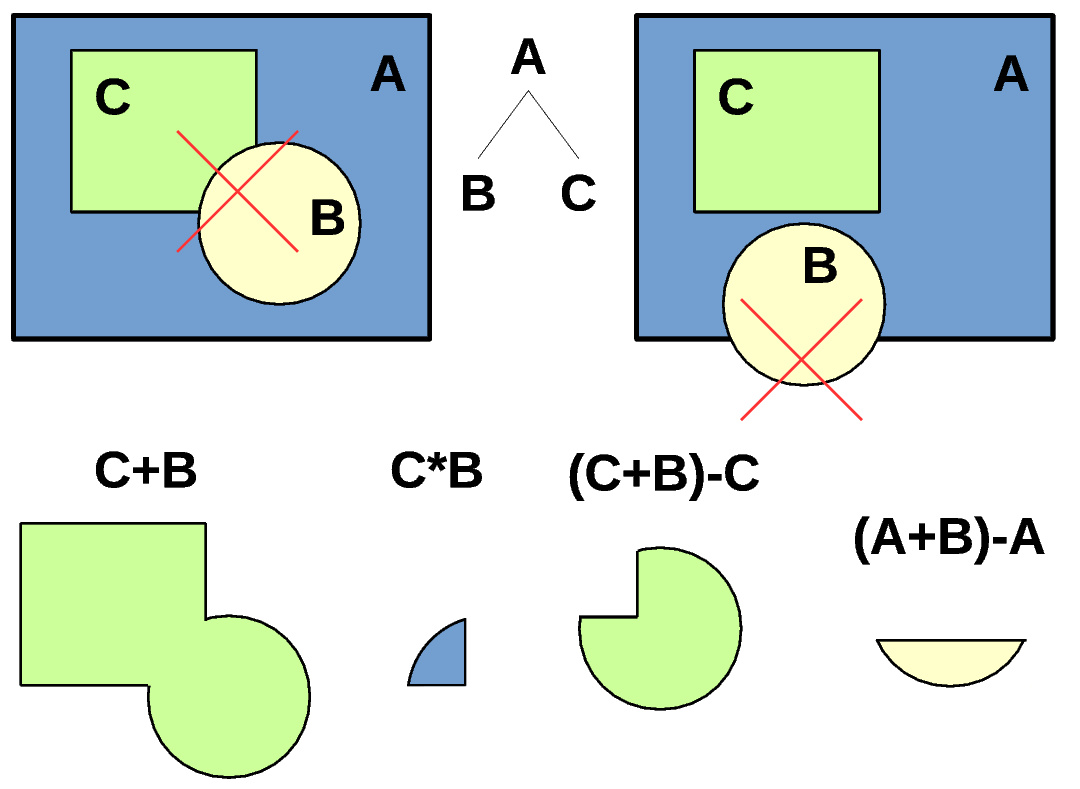
\includegraphics[width=0.6\textwidth]{pictures/Checker.png}
\caption{Логические операции для определения правильности позиционирования объёмов.}
\label{fig:CheckerOperations}
\end{figure}

Чтобы организовать проверку указанных условий, разработан специальный алгоритм и реализован в виде отдельной макропрограммы \macroname{Checker} САПР CATIA. В цикле перебираются все пары объёмов, лежащих на одном уровне, и проверяется, не пусто ли множество пересечения текущей пары. В том случае, если не пусто, то возникает событие, оповещающее, что текущая пара объёмов расположена недопустимым образом.

Более детально описанный процесс выглядит следующим образом. В силу того, что физические объёмы описываются телами детали, перебор объёмов, лежащих на одном уровне, сводится к перебору всех тел детали, кроме PartBody. Чтобы исследовать множество пересечения пары тел, создаётся новое пустое тело и копии исходных. Затем применяется Булева операция Intersect над копиями, и результат заносится в ранее созданное пустое тело. На этапе выполнения формообразования Булевой операции выдаётся возможность отследить корректность результата. С точки зрения CATIA пустое пересечение является ошибочным результатом и возникает внутренняя ошибка. Именно программный отлов и обработка этой ошибки говорит о корректности расположения объёмов. После выполнения Булевой операции результирующее тело удаляется, не оставляя таким образом никаких следов промежуточных преобразований.

Для того чтобы отследить, не выходит ли объём за пределы материнского объёма, применяется схожий подход. Отличие заключается в последовательности Булевых операций --- вместо пересечения $A*B$ двух объёмов $A$ и $B$ проверяется объём, полученный последовательностью двух операций $(A+B)-A$, где $A$ --- материнский объём, а $B$ --- дочерний. Присутствие результата операции $(A+B)-A$ говорит о том, что какая-либо часть дочернего объёма расположена за пределами материнского.

\subsubsection{\macroname{CATIA2GDML}}\label{sec:CATIA2GDML}

Конвертер \macroname{CATIA2GDML} проецирует дерево потроения MC-модели из CATIA~v5 в GDML файл. За счёт того, что правила построения MC-модели в CATIA формулировались с ориентиром на структуру, принятую в GEANT/ROOT, базовый функционал прямого конвертера заключается в том, что он создаёт в выходном GDML файле сущности, соответствующие найденным объектам в дереве построения в CATIA. Важной особенностью является то, что конвертер не обращается к самой геометрии, вся необходимая информацию содержится в дереве построение модели.

% \todo проверить ссылку на массивы
% \todo может быть что-то отсюда перенести наверх
Помимо прямолинейного отображения дерева модели в CATIA на GDML, в \macroname{CATIA2GDML} осуществляется преобразование некоторых особенностей, введённых в CATIA для упрощения процесса моделирования. Так, например, для отображения массива (см. секцию~\ref{sec:secMacroArrayMaker}), которого нет в возможностях GDML, макрос рассчитывает повороты и положения каждого вхождения и создаёт независимые дочерние объёмы в GDML.
В случае линейного массива задача проста --- положение первого вхождения определяется напрямую из значений формообразований поворотов и смещения, а за счёт того, что линейные массивы могут быть только вдоль стандартных осей, положение каждого следующего вхождения рассчитывается изменением одной координаты на величину шага.
В случае круговых массивов расчёт выполняется с применением матричных преобразований, обсуждаемых в~\ref{sec:secMatrices}.

В дереве CATIA нет обособленного списка используемых в модели материалов, поэтому для создания такого в GDML выполняется нехитрый алгоритм, который при проходе в цикле по объёмам добавляет в выходной список имя материала, если такого ещё нет.

% Цвет
В ``Builder'' реализована возможность переноса цвета объёма с помощью вспомогательного тега auxilliary в GDML файле, который позволяет добавлять произвольное поле данных к описанию логического объёма. Цвет тела в CATIA никак не отображается в дереве, поэтому для формирования тега при экспорте модели опрашиваются параметры вызуализации главного тела PartBody детали, содержащие в том числе и цвет.

\subsubsection{\macroname{GDML2CATIA}}\label{sec:GDML2CATIA}

\macroname{GDML2CATIA} выполняет процедуру, обратную \macroname{CATIA2GDML} --- проецирует GDML файл на дерево модели CATIA~v5.

% \todo дублирование мысли
В GDML отсутствует возможность определять массивы с помощью pattern (см. секцию~\ref{sec:secMacroArrayMaker}),
%Такая возможность отсутствует в GDML,
поэтому при экспорте из CATIA в GDML выполняется расчёт поворотов и сдвигов для каждого элемента массива и они представляются как отдельные, независимые дочерние объёмы. Таким образом при конвертации в обратном направлении, из GDML в CATIA, невозможно восстановить массив. Следовательно, одна из немногих (единственная \todo) операций, которые необходимо совершать после импорта геометрии из GDML в CATIA --- ручной перевод множества дочерних объёмов в массив. Обычно это очень простая процедура, и заключается она в том, что удаляются все вхождения, кроме первого, и в список формообразований первого тела добаляется pattern, которому задаются необходимые параметры и имя.

% Цвет
Аналогично прямому конвертеру, для передачи цвета автоматически выполняется дополнительная операция присвоения параметров визуализации тела если в GDML встречается тэг auxilliary.

\subsubsection{\macroname{Duplicator}}\label{sec:Duplicator}

Создание MC-модели более-менее сложной экспериментальной установки обычно требует создания нескольких вхождений параметризованных подборок с разными значениями параметров. Можно привести следующий пример. Рассмотрим детектор, состоящий из однотипных модулей, содержащих массив чувствительных объёмов (сенсоров), и какие-то другие элементы, например, платы передней электроники. Предположим, что существует несколько типоразмеров модулей, отличающихся количеством и размером сенсоров. Таким детектором может быть, например, калориметр, построенный из нескольких типов модулей, отличающихся гранулярностью --- размер чувствительного объёма увеличивается по мере удаления от пучка. Очевидно, что если типы модулей отличаются лишь значениями каких-либо переменных, то представляется возможным построить одну параметризованную модель модуля, чтобы дальше использовать её многократно для построения всего детектора. К сожалению в GEANT/ROOT нет возможности так сделать --- нужно для каждого типа иметь отдельное определение геометрии. Также это невозможно и в GDML и в CATIA.

В модели для каждой комбинации параметров, то есть для каждого модуля в нашем примере, должна существовать отдельная параметризированная подсборка. При этом имена всех объёмов должны отличаться, а наборы параметров для каждого модуля должны быть независимы. В CATIA нет возможности быстро создать копию подсборки вместе со всеми параметрами и зависимостями.

% \todo причесать
Для того, чтобы атоматизировать процесс создания такой копии используется \macroname{Duplicator}.
% Работа с \macroname{Duplicator} выполняется в 2 этапа --- размножение документов и параметров, а затем формирование формул.

Случай применения \macroname{Duplicator} описан в секции~\ref{sec:secPandaMuon}.

\subsubsection{Визуализация нескольких уровней вложенности объёмов, \macroname{MultiLevelViewer}}\label{sec:MultiLevelVis}

% \todo Разбить на два раздела - теор часть и макрос ?

Significant part of the ``CATIA-GDML geometry builder'' consists in the set of rules for the user to create Monte-Carlo compatible geometric models inside CATIA.  This set of rules makes bidirectional CATIA-GDML compatibility possible but results in a few undesired features. Probably, the most irritating one is that you can only visualize one (or two, depending on how you count them) levels of volume hierarchy at once. At the same time, CATIA has the visibility flag for each drawable object (hide/show item in the object context menu) and all visible objects are drawn in the geometry area.

В соответствии со структурой документов, определённых в ``CATIA-GDML geometry builder'', в один момент можно визуализировать только один уровень вложенности.

You can see in the specification tree that the top product contains 6 parts. Reminder --- in ``CATIA-GDML geometry builder'' we are always working in the frame of one and only top product. Each of these parts represents the description of the corresponding volume. The last part is hidden for the ease of explanation --- it has a gray-ish icon in the tree. The remaining 5 parts are visible and you can see them in the geometry area. The first two are drawn in red, next two in cyan and the ``Container'' part --- in yellow. The fact that you see the red and the cyan parts geometrically inside the yellow box does not actually mean that these volumes (``Pillar1\textunderscore vac'', ``Pillar1'', ``Pillar2\textunderscore vac'', and ``Pillar2'') are inside the ``Container''.

Now if we leave only the ``Container'' shown, you can see its shape (represented by the PartBody) and its child volumes.

\begin{figure}[H]
\begin{minipage}[c]{0.495\textwidth}
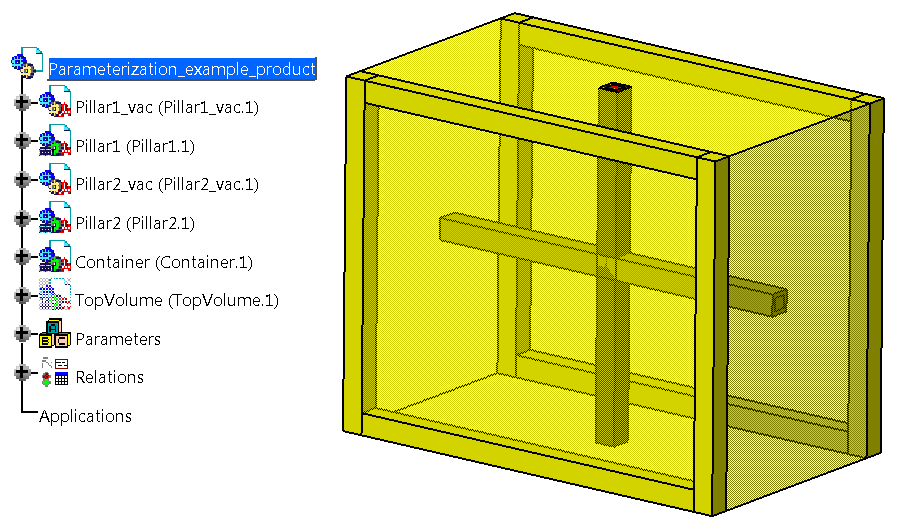
\includegraphics[width=0.95\textwidth]{pictures/MultipleLevels1.png}
\end{minipage}
\hspace{0.01\textwidth}
\begin{minipage}[c]{0.495\textwidth}
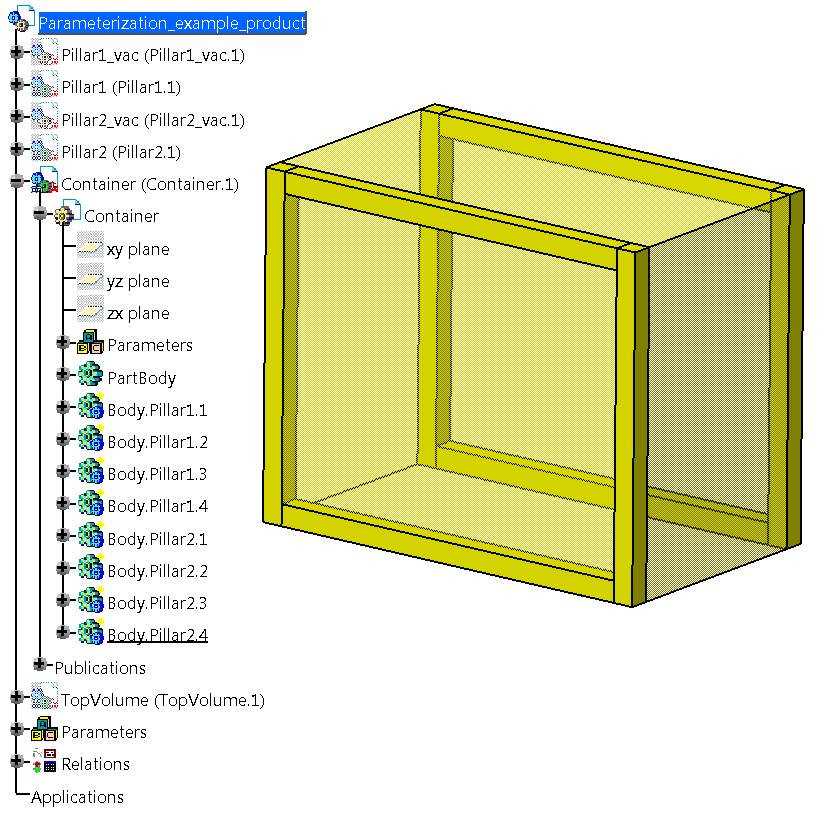
\includegraphics[width=0.95\textwidth]{pictures/MultipleLevels2.png}
\end{minipage}
\caption{Стандартная визуализация нескольких подпродуктов, находящихся на одном уровне (слева); корректная визуализация только дочерних объёмов внутри полупрозрачного материнского объёма (справа).}
\label{fig:MultiLevel1}
\end{figure}

Для того, чтобы визуализировать несколько уровней вложенности в CATIA предлагается следующий подход. Во всех документах типа CATPart, то есть для всех объёмов, все тела, обозначающие дочерние объёмы, вычитаются из главного тела PartBody. За счёт того, что в документе, описывающем материнский объём, у тел, обозначающих дочерние объёмы, есть ссылка на PartBody деталей, 

Описанная процедура автоматизирована в макропрограмме \macroname{MultiLevelViewer}.

% ================================================================================================================
%  ____  __  __ _   _                 _   _           _              
% |  _ \|  \/  | | | |     ___  _ __ | |_(_)_ __ ___ (_)_______ _ __ 
% | | | | |\/| | | | |    / _ \| '_ \| __| | '_ ` _ \| |_  / _ \ '__|
% | |_| | |  | | |_| |   | (_) | |_) | |_| | | | | | | |/ /  __/ |   
% |____/|_|  |_|\___/     \___/| .__/ \__|_|_| |_| |_|_/___\___|_|   
%                              |_|                                   
% ================================================================================================================

\subsection{Применение CATIA DMU Optimizer для построения MC-геометрии}\label{sec:CATIAoptimize}

САПР CATIA~v5 в своём составе имеет модуль DMU Optimizer, который позволяет решать задачу оптимизации. Пользователь должен сформировать критерий и определить входные параметры, возможно с допустимыми диапазонами изменения. Также необходимо выбрать один из трёх вариантов постановки задачи оптимизации --- приведение критерия к минимуму, максимуму, либо целевому значению. В качестве критерия можно выбрать существующий параметр системы CATIA~v5 либо задать аналитическое выражение над параметрами. Отдельно стоит упомянуть возможность выбора результата измерения в качестве критерия оптимизации. Например, имеется возможность средствами CATIA задать измерение расстояния или угла между камими-либо геометрическими элементами, измерение длины элемента, или даже площади или объёма элемента.

Допустим, имеется геометрическая модель объекта, которую необходимо перевести в MC-совместимый формат с упрощением геометрии, но сохранением габаритов, например подробная инженерная модель некоторого узла, упрощаемого до одного объёма. В этом случае наиболее эффективный вариант это сначала создать структуру формы с приблизительными размерами ``на глаз'', а затем с помощью оптимизации подобрать размеры примитивов. Критерий может быть составлен, например, как сумма квадратов расстояний между соответствующими точками САПР-модели и MC-модели, а входные параметры --- все или некоторые размеры примитивов, параметры позиционирования операндов.
Как второй, более сложный вариант, можно создать измерение объёма деталей узла, измерение объмов MC-геометрии и поставить задачу минизмизации их разницы. При этом, однако, нужно предварительно очень тщательно продумать структуру МС-геометрии и ограничить как можно больше параметров.

В качестве свободных параметров, помимо параметров формы, можно использовать параметры повоторов и сдвига при позиционировании дочернего объёма внутри материнского или позиционировании Булевых операндов. Возможна ситуация, когда оптимизируется только положение, но не размеры. Оптимизация имеет смысл, когда прямое измерение невозможно. Например, если положение объёма получено сложным поворотом, то практически невозможно понять, как представить этот поворот с помощью комбинации трёх последовательных поворотов вокруг фиксированных осей в требуемом порядке (Z, Y, X для объёмов и X, Y, Z для операндров). Один из вариантов решения данной ситуации --- минимизация суммы квадратов углов между соответствующими линиями САПР-модели и MC-модели. Если же поворот дочернего объёма уже задан верно, то нет смысла запускать оптимизацию для нахождения параметров сдвига. Их можно получить прямым измерением расстояния между двумя соответствующими точками. CATIA показывает кратчайшее расстояние и, если включена соответствующая настройка, компоненты вектора, которые и являются параметрами сдвига. Макропрограмма \macroname{PointToPointAligner} (см. секцию~\ref{sec:secMacroPtPAligner}) автоматизирует данную процедуру.

Алгоритмы оптимизации итерационные, что означает, что система пытается найти значения входных параметров, дающих наиболее оптимальное значение критерия, путём перебора различных комбинаций в соответствии с некоторым алгоритмом. В DMU Optimizer реализовано несколько алгоритмов оптимизации. Разные алгоритмы наиболее эффективны в разных ситуациях, поэтому стоит попробовать другой алгоритм, если оптимизация не сходится. Если в качестве критерия оптимизации задан результат измерения или аналитическое выражение с использованием результата измерения, то на каждой итерации, после изменения входных параметров, система автоматически обновляет геометрическую модель для того, чтобы рассчитать значения измерений. В связи с этим оптимизация может занять значительное время (10-20 мин.) для сложных моделей.

% Диапазон
Имеется возможность задания диапазонов изменения входных параметров оптимизации. Эта возможность бывает удобна, если есть какая-либо предварительная информация или возможно оценить значение ``на глаз''.
\todo Теоретически, наличие диапазонов входных параметров сильно упрощает работу алгоритму оптимизации. Ещё лучше, если все параметры имеют заданные диапазоны. \todo \textbf{Тут нужно как-то гладко сказать. Так-то теоретически, если заданы все диапазоны, и критериальная функция непрерывная, то гарантировано нахождение оптимума некоторыми алгоритмами. Но не факт, что теми, которые есть к CATIA.}
Очевидно, что повороты должны быть ограничены диапазоном шириной $\SI{360}{\degree}$, например от $\SI{-180}{\degree}$ до $\SI{180}{\degree}$. Если не задать диапазон, то алгоритм может пробовать различные значения, кратные $\SI{360}{\degree}$ и приводящие к одинаковому результату, что может сделать процесс оптимизации бесконечным.

% Управляющие параметры
Для управления процессом оптимизации в CATIA~v5 предусмотрено несколько управляющих параметров. Пользователь может задать максимальное количество итераций, максимальное количество итераций без улучшения, максимальное время оптимизации, и др. \todo
(Из общих сведений об оптимизации)
Широко известно, что критериальная функция часто имеет множество локальных оптимумов и один или несколько глобальных оптимумов. Это необходимо учитывать при подгоне MC-геометрии к САПР-модели с помощью DMU Optimizer. Некоторые алгоритмы оптимизации основаны на генерировании случайных чисел, поэтому имеет смысл многократно запускать оптимизацию, если результат первого прогона не является удовлетворительным. Также имеет смысл повторно запускать оптимизацию с другими начальными значениями для получения альтернативных решений. В некоторых алгоритмах уже реализован мультистарт, поэтому необходимо увеличивать максимальное допустимое время расчёта и максимально допустимое количество итераций, чтобы система могла перебрать больше вариантов.

В целом, можно сказать, что оптимизация --- это полезный инструмент, с помощью которого можно решить некоторые проблемы, не решаемые другими способами. Однако невозможно свести нахождение всех параметров MC-модели к одной задаче оптимизации, т.к. с каждым новым входным параметром вырастает сложность проблемы и время, необходимое для решения. Более того, правильно составить критерий сложнее, чем явно задать размер примитива или параметр позицирования, например с помощью измерения. \textbf{Всё-таки подавляющее большинство форм --- боксы и цилиндры, расположенные вдоль стандартных осей.}
